\documentclass[11pt]{article}

\usepackage{comment} % enables the use of multi-line comments (\ifx \fi) 
\usepackage[a4paper,margin=1cm]{geometry}
\usepackage[utf8]{inputenc}
\usepackage[ngerman]{isodate}
\usepackage{gensymb}
\usepackage{graphicx}
\usepackage{booktabs}% http://ctan.org/pkg/booktabs
\usepackage{tabularx}
\usepackage{ltablex} % Longtables with tabularx
\usepackage[x11names]{xcolor}
\usepackage{amsmath}
\usepackage{amssymb}
\usepackage{amsthm}
\usepackage{array}
\usepackage{wrapfig}
\usepackage{subcaption}
\usepackage{csquotes}
\usepackage{lscape}
\usepackage{geometry}
\usepackage{multicol}
\usepackage{bm}
\usepackage{enumitem}
\usepackage{hyperref}
\usepackage{mdframed}
\usepackage{scalerel}
\usepackage{stackengine}
\usepackage{mathtools}
\usepackage{pdfpages}

% Code highlighting
\usepackage{minted}
\surroundwithmdframed{minted}

% Be able to caption equations and float them in place
\usepackage{float}

\newmdtheoremenv{theorem}{Theorem}
\theoremstyle{definition}
\newmdtheoremenv{definition}{Definition}[section]


\geometry{a4paper, margin=2.4cm}

\newcommand\equalhat{\mathrel{\stackon[1.5pt]{=}{\stretchto{\scalerel*[\widthof{=}]{\wedge}{\rule{1ex}{3ex}}}{0.5ex}}}}
\newcommand\defeq{\mathrel{\overset{\makebox[0pt]{\mbox{\normalfont\tiny def}}}{=}}}
\newcolumntype{C}{>{\centering\arraybackslash}X}

\DeclarePairedDelimiter\abs{\lvert}{\rvert}
\DeclarePairedDelimiter\norm{\lVert}{\rVert}

\newcommand*\samplemean[1]{\overline{#1}}
\newcommand*\ev[1]{\mathrel{\text{E}\left[#1\right]}}
\newcommand*\R{\mathbb{R}}
\newcommand*\N{\mathbb{N}}
\newcommand*\Z{\mathbb{Z}}
\newcommand*\diff{\mathop{}\!\mathrm{d}}
\newcommand*\Diff[1]{\mathop{}\!\mathrm{d^#1}}
\newcommand*\Exp[1]{\mathop{\text{Exp}}\left(#1\right)}
\newcommand*\Cov[1]{\mathop{\text{Cov}}\left(#1\right)}
\newcommand*\Cor[1]{\mathop{\text{Cor}}\left(#1\right)}
\newcommand*\Var[1]{\mathop{\text{Var}}\left(#1\right)}


\setcounter{tocdepth}{3}
\setcounter{secnumdepth}{3}

\graphicspath{{./img/}}

\begin{document}
	
\title{Stochastic Modelling FS20}
\author{Pascal Baumann\\pascal.baumann@stud.hslu.ch}
\maketitle



For errors or improvement raise an issue or make a pull request on the \href{https://github.com/KilnOfTheSecondFlame/mse_summaries}{github repository}.

\tableofcontents
\newpage



\section{Introduction}

Return Value Stock Market
\begin{equation*}
	\log_{10}\left(\frac{S_t}{S_{t-1}}\right)
\end{equation*}

Despite the variety of random sources there is structure in the noise. The goal is to make meaningful predictions from these structures.

\begin{definition}
	Given the set of events $\Omega$
	\begin{enumerate}[label=\Roman*.]
		\item $P: \{\text{Events in }\Omega\}\rightarrow [0,1]$ such that $\text{E} \mapsto P(\text{E})\in[0,1]$
		\item $P(\Omega) = 1$
		\item For every sequence of mutually incompatible Events $E_i$ ($E_i\cap E_j$ if $i\neq j$)
		\begin{equation*}
			P\left(\bigcup_{i=1}^\infty E_i\right) = \sum_{i=1}^{\infty} P(E_i)
		\end{equation*}
	\end{enumerate}
	$P(\text E)$ is referred to as the probability of the event $E$.
\end{definition}

\subsection{Law of Total Probability}
\begin{minipage}{0.7\linewidth}
	Given $E \in \Omega$ and the probability $P$ on $\Omega$, $P(E)$ can be calculated for a finite partition $\{A_k\}_{1\leq k\leq n}$ of $\Omega$ as follows
	\begin{equation*}
	P(E) = \sum_{k=1}^{n} P(E|A_k)P(A_k)
	\end{equation*}
\end{minipage}
\begin{minipage}{0.3\linewidth}
	\begin{center}
		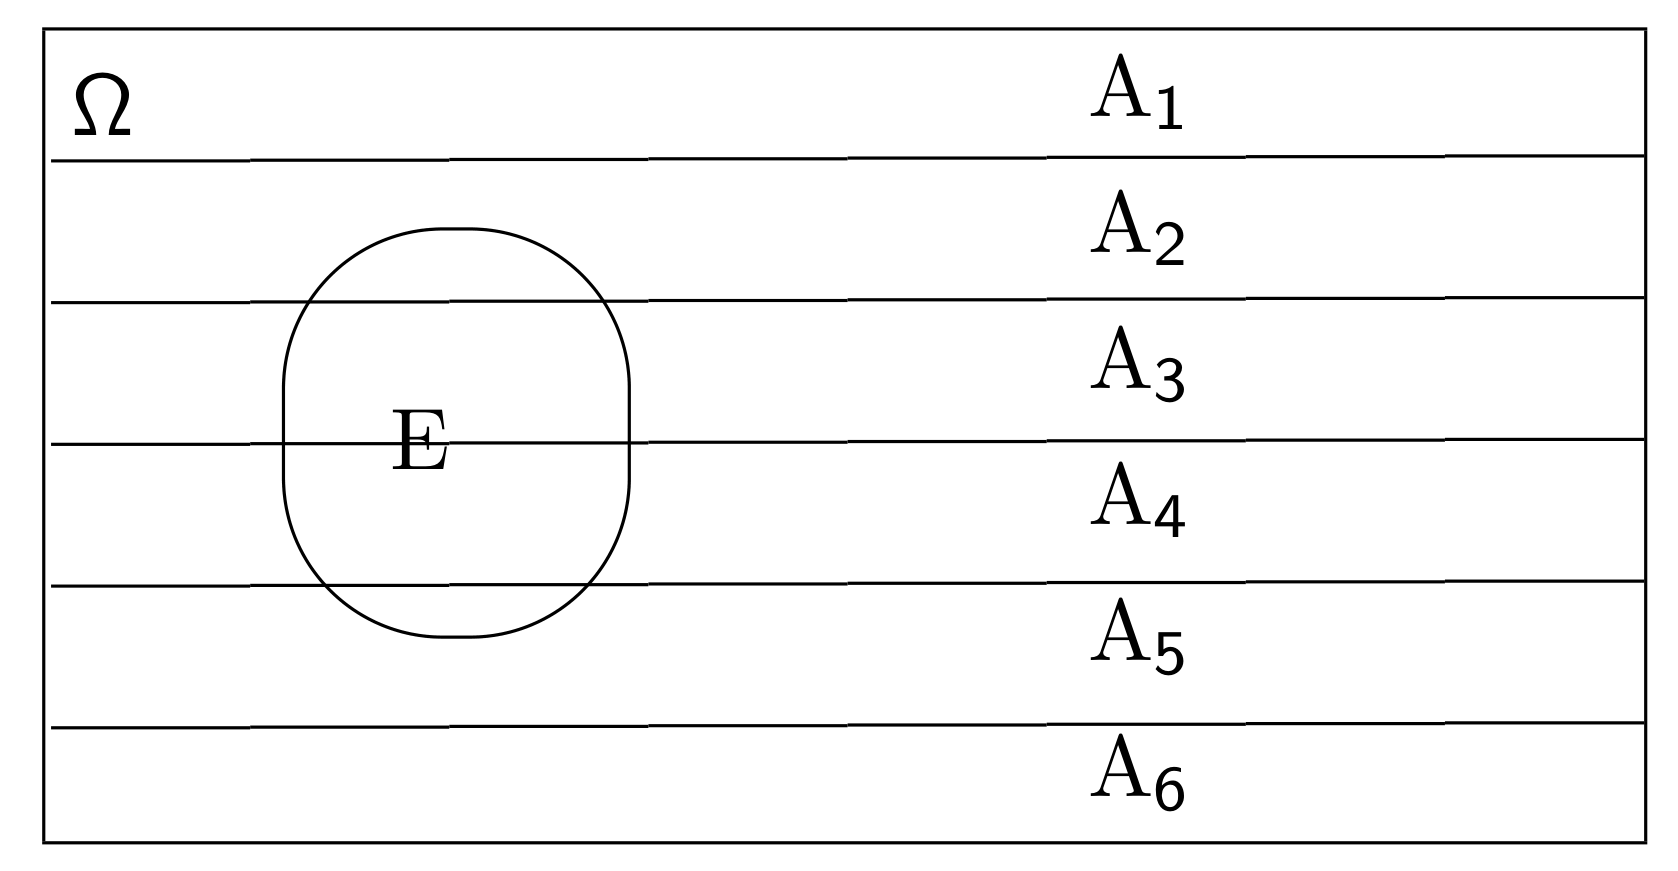
\includegraphics[width=0.9\linewidth]{img/law_total_probability}
	\end{center}
\end{minipage}

\begin{definition}
	\textbf{Bayes' Law}
	\begin{equation*}
	\textbf{P}(\textbf{A}|\textbf{E}) = \frac{P(A\cap E)}{P(E)} P \frac{P(A\cap E) P(A)}{P(E)}\frac{P(A)}{P(A)} = \frac{\textbf{P}(\textbf{E}|\textbf{A})\textbf{P}(\textbf{A})}{\textbf{P}(\textbf{E})}
	\end{equation*}
	Together with the Law of Total Probability
	\begin{equation*}
		P(A|E) = \frac{P(E|A)P(A)}{P(E|A)P(A) + P(E|\bar{A})P(\bar{A})}
	\end{equation*}
\end{definition}

\subsection{Conditional Probability}
\begin{definition}
	The conditional probability of the event $E$ given $F$
	\begin{equation*}
		P\left( E \middle| F \right) = \frac{P(E\cap F)}{P(F)}
	\end{equation*}
	Together with Bayes' law
	\begin{equation*}
		P(E|F) = \frac{P(F|E)\cdot P(E)}{P(F)}
	\end{equation*}
\end{definition}

If $A$ and $B$ are incompatible then $A\cap B = \emptyset$.
\begin{definition}
	Two events $A$ and $B$ are independent if
	\begin{equation*}
		P(A\cup B) = P(A)\cdot P(B)
	\end{equation*}
	Or equivalently (assuming $P(F)>0$)
	\begin{equation*}
		P(E|F) = P(F)
	\end{equation*}
\end{definition}

\section{Random Variables}

\begin{definition}
	A random variable $X$ is a function with values in $\R^n$, defined on the sample space $\Omega$ of a random experiment
	\begin{equation*}
		X: \Omega \rightarrow \R
	\end{equation*}
\end{definition}

\begin{tabularx}{\linewidth}{lX}
	Expectation of continuous $X$: & $\mu := E(X) = \int_{-\infty}^{\infty} x f(x) dx$\\
	Expectation of continuous $g(X)$: & $E(X) = \int_{-\infty}^{\infty} x f(x) dx$\\
	Expectation of discrete $X$: & $\mu := E(X) = \sum_{i=1}^{\infty} x_i P(X = x_i)$\\
	Expectation of discrete $g(X)$: & $E(X) = \sum_{i=1}^{\infty} g(x_i) P(X = x_i)$\\
	Estimator for $E(X)$: & $ \bar{x} = \frac{1}{n} \sum_{i=1}^{\infty} g(x_i)$
\end{tabularx}

\textbf{The expectation operator $E(\cdot)$ is a linear operator}
\begin{equation*}
E(\alpha X_1 + \beta X_2) = \alpha E(X_1) + \beta E(X_2)
\end{equation*}


\begin{tabularx}{\linewidth}{lX}
	Variance of continuous $X$: & $ E((X-\mu)^2) = \int_{\infty}^infty (x-\mu)^2 dx $\\
	Variance of discrete $X$: & $ E((X-\mu)^2) = \sum (x-\mu)^2 P(X=x_i)  $\\
	Estimator for $V(X)$: & $\sigma^2(X) = \frac{1}{n-1} \sum_{i=1}^{n}(x_i - \bar{x})^2$\\
	Estimator for k'th moment of $X$: & $M_k = \frac{1}{n}\sum_{i=1}^{n}(x_i)^k$
\end{tabularx}

The variance operator $V(\cdot)$ is not a linear operator
\begin{align*}
	V(\alpha X_1) &= \alpha^2 V(X_1)\\
	V(X_1 + X_2) &= V(X_1) + V(X_2) + \Cov{X_1,X_2}
\end{align*}
where $\Cov(\cdot)$ is the \textbf{covariance}

\begin{tabularx}{\linewidth}{lX}
	Cumulative distribution function: & $ F(x) = P(X\leq x) = \int_{-\infty}^{x}f(y)dy$\\
	Cumulative distribution function: & $ F(x) = P(X\leq x) = \sum_{x_i \leq x} P(X=x_i)$\\
	Density function: & $ f(x) = \frac{dF(x)}{dx} = \frac{d}{dx}\int_{-\infty}^{x}f(y)dy$\\
	Probability mass function: & $ P(X = x_i) = F(x_i) - F(x_{i-1})$\\
\end{tabularx}

\begin{tabularx}{\linewidth}{lX}
	Moment generating function of $X$: & $ \phi(t) := E(e^{tX}) = \int_{-\infty}^{\infty} e^{tx}f(x) dx$\\
	Moment generating function of $X$: & $ \phi(t) := E(e^{tX}) = \sum e^{tx}P(X=x_i)$
\end{tabularx}

$\phi$ is the \emph{moment generating function} because
\begin{align*}
	\dot{\phi}(0) = \left.\frac{\text{d}\phi(t)}{\text{d}t}\right|_{t=0} = \left. E(X e^{tX})\right|_{t=0} &= E(X)\\
	\phi^{(n)}(0) = \left.\frac{\text{d}^n\phi(t)}{\text{d}t^n}\right|_{t=0} = \left. E(X^n e^{tX})\right|_{t=0} &= E(X^n)
\end{align*}

\subsection{Bernoulli Random Variable}
A random variable $X$ is a Bernoulli random variable if $X$ takes on \textbf{two} values $x_1$ (success) and $x_2$ (failure) and if there exists $p\in[0,1]$ such that the probability distribution is
\begin{align*}
	P(X=x_1) &= p\\
	P(X=x_2) &= 1-p
\end{align*}

A random variable $X$ is a Binomial random variable with parameter $(\textbf{n}, \textbf{p})$, if $X$ can be written as the sum of $n$ independent and identically distributed Bernoulli variables with parameter $p$:

\begin{equation*}
	X = \sum_{k=1}^{n} X_k\quad X_k \sim \text{Bernoulli}(p)
\end{equation*}

If the $X_k$ takes on values in ${0,1}$ then $X$ takes values in ${0,1,\dots,n}$ and the probability distribution is
\begin{equation*}
	P(X=i) = \binom{n}{i} p^i(1-p)^{n-1}\quad i=0,1,\dots, n
\end{equation*}

\subsection{Poisson Random Variable}

A random variable with value in $\N_0 = {0,1,2,\dots}$ has a \textbf{Poisson distribution} with parameter $\lambda$, if for some $\lambda>0$ we have
\begin{equation*}
	P({X=i}) = \frac{\lambda^i}{i!}^{-\lambda}\quad i=0,1,2,\dots
\end{equation*}

Poisson random variables are excellent approximations for binomial random variables $\text{Binom}(n,p)$ in case $n$ is large and $p$ is small, or said differently \textbf{rare events with large trials are Poisson like events with $\lambda = np$}

\subsection{Uniform Random Variable}
A random variable $X$ taking on values in the interval $[\alpha,\beta]$ has a \textbf{uniform distribution} it its probability density function is
\begin{equation*}
	f(x) = \left\{ \begin{matrix}
	\frac{1}{\beta - \alpha}&\text{if } \alpha\leq x\leq \beta\\
	0 & \text{else}
	\end{matrix} \right.
\end{equation*}

Denoted as $X\sim \text{U}(\alpha,\beta)$.

\subsection{Exponential Random Variable}
A random variable $X$ taking on values in $\R^+$ has an \textbf{exponential distribution} with parameters $\lambda>0$ it its probability density function is
\begin{equation*}
	f_X(x) = \left\{ \begin{matrix}
	\lambda e^{-\lambda x} & \text{if } x\geq 0\\
	0 & \text{if } x< 0
	\end{matrix} \right.
\end{equation*}

Denoted as $X\sim \text{Exp}(\lambda)$.
\begin{align*}
	\text{E}(X) = \frac{1}{\lambda}\\
	\text{V}(X) = \frac{1}{\lambda^2}
\end{align*}

\subsection{Normal Random Variable}
A random variable $X$ taking on values in $\R$ has a \textbf{normal distribution} with parameters $\mu$ and $\sigma^2$ if its probability density function is

\begin{equation*}
	f(x) = \frac{1}{\sqrt{2\pi}\sigma} e^{\frac{-(x-\mu)^2 }{2\sigma^2}}\qquad -\infty<x<\infty
\end{equation*}

Denoted as $X \sim \mathcal{N}(\mu, \sigma^2)$

\subsection{Affine Transformations}
If $X\sim\mathcal{N}(\mu, \sigma^2)$ then $Y := \alpha X + \beta$ is still normally distributed, but with parameters $(\alpha\mu + \beta, \alpha^2 \sigma^2)$.

In particular if $X\sim \mathcal{N}(\mu, \sigma^2)$ then
\begin{equation*}
	Y = \frac{X-\mu}{\sigma} \sim \mathcal{N}(0,1)
\end{equation*}
Such a random variable $Y$ is said to have the \emph{standard normal distribution}. Its associated cumulative distribution function is denoted
\begin{equation*}
	\Phi(x) := \frac{1}{\sqrt{2\pi}}\int_{-\infty}^{x} e^{-\frac{y^2}{2}} dy
\end{equation*}

\section{Introduction to Stochastic Processes}
\subsection{Covariance}
A random vector $(X,Y)$ is known if:
\begin{enumerate}[label=(\alph*)]
	\item the joint probability mass function in case of discrete random variables $X$ and $Y$ is known
	\begin{equation*}
		p(x,y) = P(X=x,Y=y)\quad \text{for all values $x$ and $y$}
	\end{equation*}
	\item the joint probability density function in case of continuos random variables $X$ and $Y$ is known
	\begin{equation*}
		P(X\in [a,b], >\in [c,d]) = \int_{a}^{b}\int_{d}^{c} f(x,y)\diff y\diff x\quad \text{for all } a,b,c,d
	\end{equation*}
\end{enumerate}
For any two random variables $X$ and $Y$, th joint cumulative probability distribution is given by
\begin{equation*}
	F(a,b) = P(X\leq a, Y\leq b)\quad -\infty < a, b<\infty
\end{equation*}

\begin{equation*}
	\Cov{X,Y} = \ev{(X-\ev{X})(Y-\ev{Y})} = \ev{XY} - \ev{X}\ev{Y}
\end{equation*}
In the discrete case this definition reduces to
\begin{equation*}
	\Cov{X,Y} = \sum_{x_i,x_j} (x_i - \ev{X})(y_i - \ev{Y})\cdot P(X=x_i,Y=y_i)
\end{equation*}
and in the continuous case
\begin{equation*}
	\Cov{X,Y} = \int_{-\infty}^{\infty}\int_{-\infty}^{\infty}(x-\ev{X})(y-\ev{Y})\cdot f(x,y)\diff x\diff y
\end{equation*}
The correlation coefficient $\rho$ is the normalised covariance
\begin{equation*}
	\rho := \frac{\Cov{X,Y}}{\sqrt{\Var{X}}\sqrt{\Var{Y}}}
\end{equation*}

\subsection{Correlation}
$X$ and $Y$ are \textbf{positively} correlated if $\Cov{X,Y} > 0$ and \textbf{negatively} correlated if $\Cov{X,Y} < 0$. $X$ and $Y$ are not correlated if $\Cov{X,Y} = 0$, that is $\ev{XY} = \ev{X} + \ev{Y}$ in which case $\Var{X + Y} = \Var{X} + \Var{Y}$.

\subsection{The Bivariate Normal}

Density function of $(X_1,X_2)$
\begin{align*}
	f_{X_1, X_2}(x_y,x_2) &:= \frac{1}{2\pi\sigma_1\sigma_2\cdot\sqrt{1-\rho^2}}\\
	& e^{-\frac{1}{2(1-\rho^2)}} \left[ \left(\frac{x_1 - \mu_1}{\sigma_1}\right)^2 - 2 \rho\frac{x_1 - \mu_1}{\sigma_1}\frac{x_2- \mu_2}{\sigma_2} - \left(\frac{x_2 - \mu_2}{\sigma_2}\right)^2 \right]
\end{align*}

%TODO Marginal densities

\subsection{The Multivariate Normal}
$\textbf{X}$ follows a multivariate normal with mean vector $\bm{\mu}$ and covariance matrix $\textbf{C}$ if the density function of $\textbf{X}$ can be written as
\begin{equation*}
	f_{\textbf{X}}(\textbf{x}) = \frac{1}{(2\pi)^{\frac{n}{2}}\sqrt{\det \textbf{C}}} e^{- \frac{1}{2} (\textbf{x}-\bm{\mu})^T \textbf{C}^{-1}(\textbf{x}-\bm{\mu})}
\end{equation*}
And the notation is $\textbf{X}\sim \mathcal{N}(\bm{\mu}, \textbf{C})$

\subsection{Law of Large Numbers}
\begin{theorem}
	Let $X_1, X_2, \dots$ be a sequence of independent and identically distributed random variables with $\ev{X} = \mu$. Then, with probability 1,
	\begin{equation*}
		\frac{X_1 + X_2 + \dots + X_n}{n} \longrightarrow \mu \qquad\text{as }\mu\rightarrow\infty
	\end{equation*}
\end{theorem}

% TODO Central Limit Theorem 

\section{Stochastic Processes}

\begin{definition}
	Let $P$ be a probability function on the sample space $\Omega$. A stochastic process $X = \left\{ X_t | t\in \mathbb{T} \right\}$ with state space $S$ is a collection of random variables with values in the set $S$
	\begin{equation*}
		X_t : \Omega \rightarrow S\qquad t\in\mathbb{T}
	\end{equation*}
	where $\mathbb{T}$ is an ordered set, called the index set of the process.
\end{definition}

\pagebreak
\subsection{Classification}
\begin{equation*}
	X_t : \Omega \rightarrow S\qquad t\in\mathbb{T}
\end{equation*}
\begin{tabularx}{\linewidth}{|X||c|c|}
	\hline
	& $\bm{\mathbb{T}}$ \textbf{discrete} & $\bm{\mathbb{T}}$ \textbf{continuous}\\
	\hline
	\hline
	$\bm{S}$ \textbf{discrete} & random walk & Poisson process\\
	\hline
	$\bm{S}$ \textbf{continuous} & time series & Brownian motion\\
	\hline
\end{tabularx}

\begin{definition}
	A stochastic process $X$ is \textbf{strict sense stationary}, if the finite dimensional distribution function is invariant under time shift.
\end{definition}

\begin{definition}
	A stochastic process $X$ is \textbf{wide sense stationary}, if the mean $E(X_t) = m$ is constant and if the autocorrelation function $R_X(t_1,t_2)$ only depends on the difference $t_2-t_1$.
\end{definition}

\begin{definition}
	The \textbf{(power) spectral density} of a wide sense stationary stochastic process $X$ is the Fourier transform $S_X(k)$ of its autocorrelation function $R_X(t)$
	\begin{equation*}
		S_X(k) = \int_{-\infty}^{\infty}e^{-jkt} R_X(t)\diff{t}
	\end{equation*}
\end{definition}

\section{Markov Chain}
The stochastic process $X$ has the Markov property if a step $X(t_n)$ is only dependent on the preceding step $X(t_{n-1})$
\begin{equation*}
	P\left(X(t_n)\leq x_n \middle| \{X_t\}_{t\leq t_{n-1}} \right) = P\left(X(t_n)\leq x_n \middle| X(t_{n-1}) \right)\qquad\text{for }t_{n-1}<t_n
\end{equation*}
A sequence of integer valued random variables $X_0, X_1,\dots$ is called a Markov chain if for $n \geq 1$
\begin{equation*}
	P\left( X_{n+1}=x_{n+1} \middle| X_{n}=x_{n},\dots,X_{0}=x_{0} \right) = \underbrace{P\left( X_{n+1}=x_{n+1} \middle| X_{n}=x_{n} \right)}_{\text{transition probability}}
\end{equation*}

The conditional probabilities $P\left(X_{k+1}=j \middle| X_k = i\right)$ of a Markov chain $X$ are called transition probabilities. A Markov chain is called time-homogenous, if the transition probabilities do not depend on time $k$ and the following notation is used
\begin{equation*}
	p_{ij} = P\left(X_{k+1}=j\middle| X_k = i\right)
\end{equation*}
for homogeneous transition probabilities. The associated matrix, indexed by the state space $S = \{1,2,\dots,n\}$ is the transition matrix
\begin{equation*}
	\bm{P} = \begin{pmatrix}
	p_{11} & \dots & p_{1n}\\
	\vdots & \ddots & \vdots \\
	p_{n1} & \dots & p_{nn}
	\end{pmatrix}
\end{equation*}
\begin{center}
	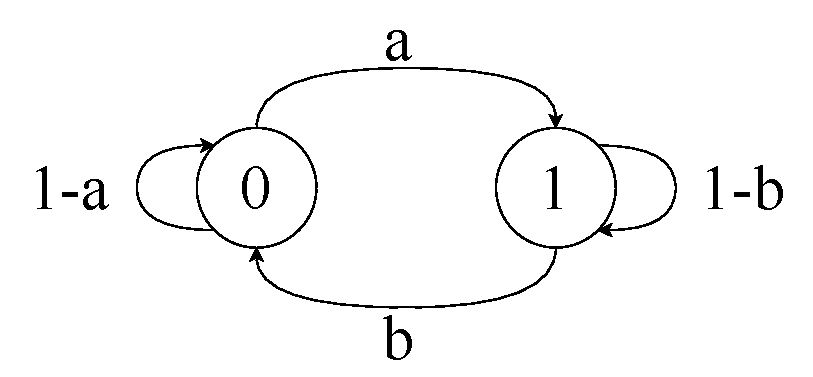
\includegraphics[width=0.6\linewidth]{img/discrete_markov_chain}
\end{center}
This diagram says that the state space is the finite set ${0,1}$, and that
\begin{equation*}
	\bm{P} = \begin{pmatrix}
	1-a & a\\
	b & 1-b
	\end{pmatrix}
\end{equation*}
\subsection{The Chapmann-Kolmogorov Equations}
Define the probability of going from state $i$ (at time zero) to state $j$ in $m$ steps
\begin{equation*}
	p_{ij}^{(m)} = P\left( X_m = j \middle| X_0 = i \right)
\end{equation*}
In particular
\begin{equation*}
	p_{ij}^{(1)} = p_{ij}\text{ and } p_{ij}^{(0)} = \delta_{ij} = \left\{\begin{matrix}
	1 & i=j\\
	0 & i\neq j
	\end{matrix}
	\right.
\end{equation*}
The $m$-step transition probabilities satisfy the Chapman-Kolmogorov equation
\begin{equation*}
	p_{ij}^{(n+m)} = \sum_{k} p_{ik}^{(n)} p_{kj}^{(m)}
\end{equation*}




\end{document}